\documentclass[../main]{subfiles}

\begin{document}

\section{Energetics} 

	\subsection{Chemical Reactions and Energy}

	\scidef{Chemical Energetics}{Chemical Energetics is the study of energy changes that occurs during reactions and phase changes.}

	\scidef{State Function}{A State Function is a function whose values only depend on the state of a system, rather than the pathway used to reach a state.}

	\scieqn{State Function Change}{The change in a state function \(\Delta f\) is obtained using its beginning \(f_\text{initial}\) and final \(f_\text{final}\) values by the equation:}{\Delta f = f_\text{final} - f_\text{initial}}

	\subsubsection{Enthalpy}

	\scidef{Enthalpy}{The Enthalpy \(H\) of a substance is a quantification of its energy content. Substances with lower \(H\) or lower enthalpy have less energy and are more stable. Enthalpy is a state function. Measured in \si{\J}}

	Absolute enthalpy cannot be obtained, but rather the change in enthalpy \(\Delta H\) has a real value and is calculated like a state function.

	\scidef{Endothermic}{An Endothermic reaction is one where energy is released to the surroundings, i.e. \(\Delta H > 0\)}

	\scidef{Exothermic}{An Exothermic reaction is one where energy is released to the surroundings, i.e. \(\Delta H < 0\)}

	\scidef{Activation Energy}{Activation Energy \usub{E}{A} is the amount of energy required for reactant particles to possess before they can collide successfully to form products.}

	As particles form bonds, they become more stable and release energy, whereas when breaking bonds particles are excited and absorb energy. Hence, bond formation is typically exothermic and bond breaking is endothermic. \\

	Exothermic reactions are energetically feasible and are more likely to occur. However, energetic stability is insufficient to assess the speed of which reactions will happen, which can be very slow (like \ch{C_{Diamond} -> C_{Graphite}})

	\subsection{Energy Profile Diagram}

	Energy profile diagrams describe the potential energy stored in a substance as a reaction progresses, showing the relative energy levels of its reactants, products and the activation energy required.

	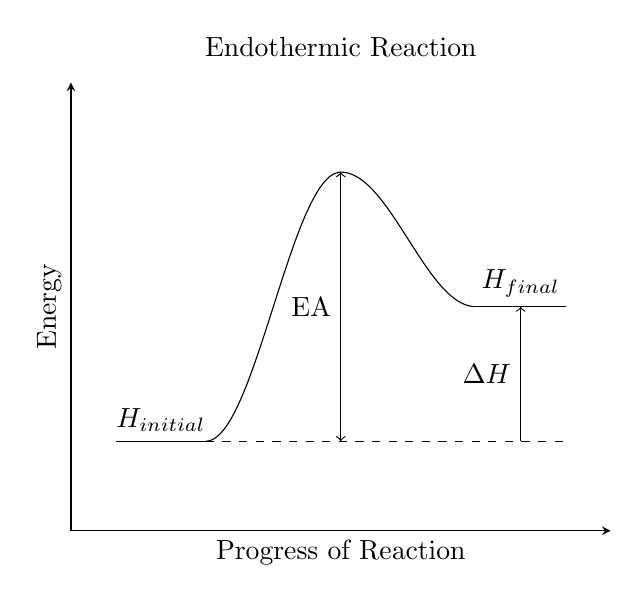
\begin{tikzpicture}
	\begin{axis}[
		axis x line=bottom,
		axis y line=left,
		xmin=0,xmax=6,ymin=0,ymax=5,
		xlabel={Progress of Reaction},
		ylabel={Energy},
		ticks=none,
		title={Endothermic Reaction}
	]
	\addplot [] coordinates { (0.5,1) (1.5,1) }
		node [pos=0.5,anchor=south] {\(H_\text{initial}\)};
	\addplot [] coordinates { (4.5,2.5) (5.5,2.5) }
		node [pos=0.5,anchor=south] {\(H_\text{final}\)};
	\addplot [dashed] coordinates { (1.5,1) (5.5,1)};
	\addplot [samples=100,domain=1.5:3] {2.5+1.5*sin(x*120+90)};
	\addplot [samples=100,domain=3:4.5] {3.25+0.75*sin(x*120+90)};
	\draw [->] (5,1) -- (5,2.5)
		node [pos=0.5,anchor=east] {\(\Delta H\)};
	\draw [<->] (3,1) -- (3,4)
		node [pos=0.5,anchor=east] {\usub{E}{A}};
	\end{axis}
	\end{tikzpicture}

	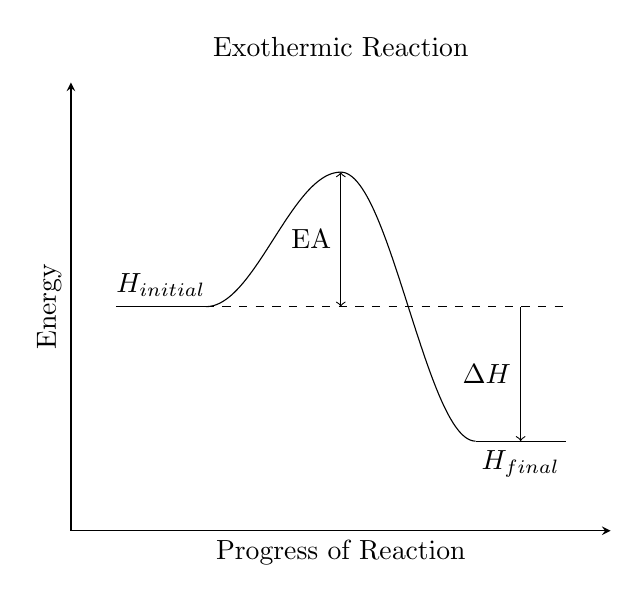
\begin{tikzpicture}
	\begin{axis}[
		axis x line=bottom,
		axis y line=left,
		xmin=0,xmax=6,ymin=0,ymax=5,
		xlabel={Progress of Reaction},
		ylabel={Energy},
		ticks=none,
		title={Exothermic Reaction}
	]
	\addplot [] coordinates { (0.5,2.5) (1.5,2.5) }
		node [pos=0.5,anchor=south] {\(H_\text{initial}\)};
	\addplot [] coordinates { (4.5,1) (5.5,1) }
		node [pos=0.5,anchor=north] {\(H_\text{final}\)};
	\addplot [dashed] coordinates { (1.5,2.5) (5.5,2.5)};
	\addplot [samples=100,domain=1.5:3] {3.25+0.75*sin(x*120+90)};
	\addplot [samples=100,domain=3:4.5] {2.5+1.5*sin(x*120+90)};
	\draw [<-] (5,1) -- (5,2.5)
		node [pos=0.5,anchor=east] {\(\Delta H\)};
	\draw [<->] (3,4) -- (3,2.5)
		node [pos=0.5,anchor=east] {\usub{E}{A}};
	\end{axis}
	\end{tikzpicture}

	Note that the arrows for \usub{E}{A} have two arrowheads while \(\Delta H\) only has one. The number of peaks in energy of a molecule indicate an intermediate step in the mechanism.

	\subsection{Standard Enthalpy Definitions}

	\scidef{Standard Conditions}{Standard Conditions (subscript \plimsoll, pronounced naught and symbol is called a plimsoll) refer to situations where temperature is \SI{298}{\K}, pressure is \SI{1}{\bar} and solutions have concentration \SI{1}{\mol\per\dm\cubed}. Standard conditions \(\neq\) s.t.p or r.t.p.}

	\scidef{Standard States}{Standard States are the physical and chemical states at which a substance is most stable at standard conditions. Standard states of substances with the same chemical formula follow their most stable sample (\usub{C}{graphite} rather than \usub{C}{diamond}, \ch{H2O} at liquid rather than gas).}

	Note for each reaction that \(\Delta H\) is defined for \SI{1}{\mol} of the reaction rather than of a product or reactant if not stated, as well as the physical states of all substances. \\

	Definitions of standard enthalpies follow the general form of:

	\begin{center}
	The standard enthalpy change of \textbf{[process]} is the energy \textbf{(changed/released/absorbed)} when \textbf{[amount to be observed]} of \textbf{[specific substance with physical state]} is \textbf{[description of process]} under conditions of \textbf{[temperature, pressure, concentration and other conditions]}.
	\end{center}

	\subsubsection{List of Standard Enthalpies}

	\begin{description}

		\item[Standard enthalpy change of reaction] \(\Delta H_\text{r}^\plimsoll\) is the energy change in a reaction when one mole of reaction occurs with stated quantities of a reaction under standard conditions.
		
		\item[Standard enthalpy change of formation] \(\Delta H_\text{f}^\plimsoll\) is the energy released when one mole of substance is formed from its elements under standard conditions.
		
		\item[Standard enthalpy change of combustion] \(\Delta H_\text{c}^\plimsoll\) is the energy released when one mole of substance is completely burnt under standard conditions.
		
		\item[Standard enthalpy change of neutralization] \(\Delta H_\text{neut}^\plimsoll\) is the energy change when one mole of \ch{H2O} is formed through reacting an acid and a base under standard conditions. \\
		Neutralization between strong acid and strong base typically has enthalpy change of \SI{-57.3}{\kJ\per\mol}. \\
		Neutralization can be endothermic in the case of a weak acid or base, as the endothermic disassociation of \ch{H+} a nd \ch{OH-} combined with the exothermic hydration of ions may result in a net endothermic effect which is larger than the energy released due to formation of \ch{H2O}, hence it may be endothermic.

		\item[Standard enthalpy change of atomization] \(\Delta H_\text{atom}^\plimsoll\) is the energy required for when gaseous element molecules are atomized into one mole of gaseous atoms or one mole of gaseous compound is atomized into constituent gaseous atoms.
		
		\item[Bond Dissociation Energy] BDE is the energy required to break one mole of a particular bond in a compound when the compound is in gaseous state.
		
		\item[Bond Energy] BE is the average energy required to break one mole of a type of bond between two atoms. \\
		BE is obtained when BDE is averaged out.
		
		\item[Ionization Energy] IE is the energy required to form one mole of gaseous electrons and one mole of charged gaseous atoms from one mole of gaseous atoms.
		
		\item[Electron Affinity] EA is the energy change when one mole of gaseous atoms acquire one mole of gaseous electrons. \\
		Note that the first EA can be exothermic or endothermic, but the second EA is endothermic because electrons are being introduced to a negatively charged species and will experience repulsion.
		
		\item[Lattice Energy] LE is the amount of energy released when gaseous cation and anion  react to form one mole of solid ionic compound under standard conditions.
		
		\item[Standard enthalpy change of hydration] \(\Delta H_\text{hyd}^\plimsoll\) is the energy released when one mole of gaseous ion is hydrated under standard conditions. \\
		\(\Delta H_\text{hyd}^\plimsoll\) is proportional to the charge density of an ion, i.e. \(\Delta H_\text{hyd}^\plimsoll \propto | \frac{q}{r} |\)
		
		\item[Standard enthalpy change of solution] \(\Delta H_\text{soln}^\plimsoll\) is the energy change when one mole of substance is completely dissolved in solvent to form an infinitely dilute solution under standard conditions.

	\end{description}

	When asked to define standard enthalpies in a question, ensure that responses are defined with respect to reactants specified in the question rather than just a generic definition. Answer with context.

	\subsection{Energy Cycles}

	\scidef{Hess' Law}{Hess' Law states that the enthalpy change of a reaction is determined by its initial and final states of the system and independent of the pathways taken. i.e. Enthalpy is a state function.}

	Given a list of \(\Delta H\) and the data from the information booklet, \(\Delta H\) of other reactions can be found by exploiting this rule. No matter how many steps of a reaction is taken, so long as the reactants and products are the same, the total \(\Delta H\) will be the same. \\

	When drawing cycles:
	\begin{itemize}
		\item Always show state symbols of substances
		\item Label reactions/arrows with the correct \(\Delta H_\text{subscript}\), value of enthalpy change and introduced or removed elements (and their state) if there are any
		\item Only use \plimsoll when data given is applicable to standard conditions
		\item Ensure that all introduced elements are also removed at some point in a cycle
		\item Write ``By Hess' Law,'' before calculations of enthalpy change.
		\item As a worst case scenario, ensure that cycles are complete in order to salvage marks.
		\item Be especially careful with BE values; For \ch{3/2 Cl2 -> 3 Cl}, \(\Delta H\) is \ch{3/2 BE(Cl-Cl)} rather than \ch{3 BE(Cl-Cl)}
	\end{itemize}

	\subsubsection{Energy Cycle Shortcuts}

	Given the \(\Delta H_\text{f}\) or \(\Delta H_\text{c}\) of both products and reactants, \(\Delta H_\text{r}\) of a reaction can be calculated with:

	\scieqn{\(\Delta H_\text{r}\) given \(\Delta H_\text{f}\) of products and reactants}{}{\Delta H_\text{r} = - \Delta H_\text{f}(\text{reactants}) + \Delta H_\text{f} (\text{products})}
	\scieqn{\(\Delta H_\text{r}\) given \(\Delta H_\text{c}\) of products and reactants}{}{\Delta H_\text{r} = + \Delta H_\text{f}(\text{reactants}) - \Delta H_\text{f} (\text{products})}

	\subsubsection{Energy Level Diagrams}

	Energy level diagrams are a special type of energy cycle which are drawn with energy as a vertical axis where each state of a set of substances occupy a vertical position.

	In addition to the above, when drawing energy level diagrams:
	\begin{itemize}
		\item Label the vertical axis and the ``/\si{\kJ\per\mol}'' unit.
		\item Attempt to maintain proportion between changes in enthalpy: larger \(\Delta H\) should have a larger vertical gap than smaller \(\Delta H\)
		\item One arrow corresponds to one kind of reaction with one \(\Delta H\) value, do not have multiple reactions occurring at once.
		\item Up arrows show endothermic reactions, down arrows exothermic
		\item Label a zero at the energy level where all reactants are at its standard state.
	\end{itemize}

	For drawing energy level diagrams to obtain LE of a substance, follow the steps:
	\begin{enumerate}
		\item Draw standard state of metal and nonmetal, label as zero energy.
		\item Draw state of ionic solid and arrow from standard state to ionic solid for formation of ionic solid.
		\item Draw state of gaseous atoms of metal and nonmetal from standard state.
		\item Draw state of cations and anions from gaseous atoms. Note that cations need to be formed first. Gaseous \ch{e-} also needs to be included.
		\item Join cations and anions to ionic solid with arrow labeled as LE.
	\end{enumerate}

	Note that the first \usub{E}{A} may be negative for the nonmetal and its corresponding vertical position with respect to the other states needs to be calculated and shown properly. If it dips below a previous state it should be shown properly.

	\subsection{Lattice Energy}

	Theoretical calculations for lattice energy can be obtained through using the previously shown formula of \(| \text{LE} | \propto | \frac{q_+ \times q_-}{r_+ + r_-} | \). This obtains values similar to experimentally obtained results for compounds which are mostly ionic. However, partial covalent character in some ionic compounds (usually involving transition metals) causes measured LE to have a discrepancy with the theoretical equation, where partial covalent character strengthens the bond between anions and cations, causing an increase in LE.

	\subsection{Solubility}

	The process of dissolving an ionic solid involves two steps: the endothermic disassociation of ionic bonds between the solid followed by the exothermic hydration of the ions due to the formation of ion-dipole interactions. Applying Hess' Law:

	\scieqn{Standard Enthalpy of Solution}{For a ionic solid MX:}{ \Delta H_\text{soln}^\plimsoll (\ch{MX}) = \Delta H_\text{hyd}^\plimsoll (\ch{M+}) + \Delta H_\text{hyd}^\plimsoll (\ch{X-}) - LE (\ch{MX})}

	Ionic solids are more likely to be soluble if \(\Delta H_\text{soln}^\plimsoll\) is negative, where the energy released by hydration is sufficient to compensate for the lattice dissociation energy required to break down the ionic solid.

	\subsection{Entropy}

	\scidef{Entropy}{Entropy is the measure of disorder of a system. A system with higher entropy has more ways to organize itself.}

	Zero entropy is defined as the entropy of any substance at absolute zero. For the purposes of chemical energetics, entropy is treated as a state function where change in entropy is derived from comparing its initial and final states. Negative entropy change indicates that the final state is more ordered, while a positive entropy change indicates that the final state is more disordered.

	\subsubsection{Entropy Changes}

	An \textbf{increase in the number of gas particles in a system} increases the entropy of a system as an increase in gas particles creates an increase in particles in random motion, hence reactions which have a net increase of gas particles have a positive entropy change. \\

	\textbf{Mixing of particles} increases entropy as there are more ways to organize particles. Mixing gas particles causes these particles to occupy a larger container, allowing them more ways to be arranged in the larger volume. Mixing soluble liquid particles cause these liquid particles to have greater disorder than their unmixed state. \\

	\textbf{Dissolution of ionic solids in water} can cause both increases and decreases in entropy. Disruption of the ordered ionic lattice structure which causes ionic solids to lose their orderly form increases entropy significantly as they are free to move about the solvent, however there is also a decrease in entropy due to the process of hydration as ion-dipole interactions between water and ions puts these particles into an orderly arrangement. For \ch{NaCl},the dissolution process results in a net increase in randomness as breaking of ionic structure is more predominant than the process of hydration. For \ch{CaSO4},the dissolution process decreases entropy as the process of hydration is more predominant than breaking of ionic structure. \\

	\scidef{Maxwell-Boltzmann Distribution}{The Maxwell-Boltzmann Distribution graph is a plot of number of molecules with a given energy level against kinetic energy. Though the temperature of a substance is constant, its individual particles still have differing energy levels. Increasing the temperature of a substance will broaden the Maxwell-Boltzmann Distribution and also shift the peak lower and to the right.}

	An \textbf{increase in temperature} results in an increase in entropy. As temperature increases, there is a broadening of the Maxwell-Boltzmann distribution of the particles, providing more energy states which any individual particle can hold at one point in time and hence causing an increase in entropy. \\

	State changes from solid to liquid to gas cause an increase in entropy, since the structural order in a solid is destroyed by melting into a liquid and since changes to the gaseous state are accompanied with a large increase in volume. The entropy in a similar amount of gas is significantly higher than that of a liquid, which is higher than that of a solid.

	\subsection{Gibbs Free Energy}

	\scidef{Standard Gibbs Free Energy Change}{The Standard Gibbs Free Energy Change \(\Delta G^\plimsoll\) of a reaction is the overall change in the total energy content of a reaction, once accounted for both changes in enthalpy and changes in entropy.}

	\scieqn{Standard Gibbs Free Energy Change}{For the enthalpy change \(\Delta H^\plimsoll\), entropy change \(\Delta S^\plimsoll\) and current temperature \(T\) of a reaction, the Standard Gibbs Free Energy Change \(\Delta G^\plimsoll\) of a reaction is given as:}{\Delta G^\plimsoll = \Delta H^\plimsoll - T \Delta S^\plimsoll }

	Note that in most calculations \(\Delta H\) is in \si{\kJ} while \(\Delta S\) is in \si{J}, do remember to convert units. \\

	Note that in most cases where reactions take place in standard conditions, all \(\Delta G\), \(\Delta H\) and \(\Delta S\) values should be followed by a superscript \plimsoll to indicate standard conditions or the use of values obtained at standard conditions, despite temperature being different. \(\Delta H^\plimsoll\) and \(\Delta S^\plimsoll\) are assumed to not vary with different temperature. When in doubt, follow the notation of the question.

	\subsubsection{Thermodynamic Feasibility}

	\scidef{Thermodynamic Spontaneity}{A Thermodynamically Spontaneous reaction is a irreversible reaction that can occur without any external assistance in terms of energy input, involving a system which moves from a unstable to a stable state.}

	\scidef{Endergonic}{An Endergonic reaction has a positive \(\Delta G\) value and is not thermodynamically spontaneous.}

	\scidef{Exergonic}{An Exergonic reaction has a negative \(\Delta G\) value and is thermodynamically spontaneous.}

	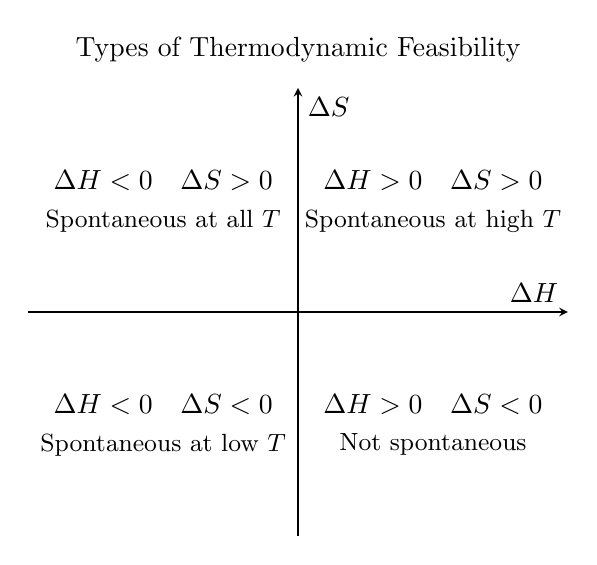
\begin{tikzpicture}
	\begin{axis}[
		axis x line=center,
		axis y line=center,
		xmin=-3,xmax=3,ymin=-3,ymax=3,
		xlabel={\(\Delta H\)},
		ylabel={\(\Delta S\)},
		ticks=none,
		title={Types of Thermodynamic Feasibility}
	]
	\node [anchor=north east] (0,0) {0};
	\node [anchor=south] at (-1.5,1.5) {\(\Delta H < 0 \quad \Delta S > 0\)};
	\node [anchor=north] at (-1.5,1.5) {\small Spontaneous at all \(T\)};
	\node [anchor=south] at (1.5,1.5) {\(\Delta H > 0 \quad \Delta S > 0\)};
	\node [anchor=north] at (1.5,1.5) {\small Spontaneous at high \(T\)};
	\node [anchor=south] at (-1.5,-1.5) {\(\Delta H < 0 \quad \Delta S < 0\)};
	\node [anchor=north] at (-1.5,-1.5) {\small Spontaneous at low \(T\)};
	\node [anchor=south] at (1.5,-1.5) {\(\Delta H > 0 \quad \Delta S < 0\)};
	\node [anchor=north] at (1.5,-1.5) {\small Not spontaneous};
	\end{axis}
	\end{tikzpicture}

	To explain the thermodynamic feasibility of a reaction:
	\begin{enumerate}
		\item State and explain sign of \(\Delta H\)
		\item State and explain sign of \(\Delta S\)
		\item Comment on sign on \(\Delta G\):
		\begin{description}
			\item[(Not) Spontaneous at all T] is because \(\Delta H\) and \(T \Delta S\) both have the same sign, hence \(\Delta G\) will be (positive/negative) regardless of T
			\item[T dependent] is because at low T \(\Delta G\) is (positive/negative) since \_ outweighs \_, but at high T \(\Delta G\) is (negative/positive) since \_ outweighs \_.
		\end{description}
	\end{enumerate}

	\subsection{Experimental Energetics}

	Experimental methods to find \(\Delta H\) of reactions are in syllabus.

	\subsubsection{Highest Reading Method}

	This method involves the derivation of enthalpy change by direct reading of temperature change. A reaction is conducted in an insulated environment with known volumes and amount of reactants. The maximum/minimum temperature reading of the system is then read and used to calculate \(\Delta H\) through calculating the heat capacity of the system, using temperature change to find the total amount of heat change and finally calculating heat change per unit of reaction. \\

	\scieqn[gathered]{Highest Reading Method}{For a resultant volume of system \(V\), density of water \(\rho_\text{\ch{H2O}}\), specific heat capacity of water \(c_\text{water}\), measured temperature change \(\Delta T\) which then gives the amount of heat transfer \(q\), and finally amount of reaction \(n\), the enthalpy of a reaction \(\Delta H\) is given by the equations:}{
		q = mc \Delta T \\
		\Delta H = -\frac{q}{n}
	}

	This experiment assumes that:
	\begin{itemize}
		\item There is negligible heat loss to surroundings
		\item The resultant solution is infinitely dilute: its density and its heat capacity  is equal to that of water
	\end{itemize}

	\subsubsection{Graph Method}

	This method involves the derivation of enthalpy change by estimating temperature change and compensating for heat loss through using a graphical method. A reaction is conducted in an insulated environment with known volumes and amount of reactants, and the temperature of the system is taken at regular intervals before and after reaction takes place. A graph of temperature against time is plotted, and the temperature change reading is obtained through intersecting two lines: one line of \(x = \text{time of start of reaction}\) and one best fit line of the temperature readings after reaction takes place and temperature change due to reaction is complete. This experiment, after graphing, uses similar equations to the Highest Reading method to obtain \(\Delta H\).\\

	This experiment assumes that:
	\begin{itemize}
		\item Heat loss to surroundings is at a constant rate and is accounted for via extrapolation
		\item Reaction is instantaneous
		\item The resultant solution is infinitely dilute: its density and its heat capacity  is equal to that of water
	\end{itemize}

	\subsection{Exam Technique}

	When a question specifies ``with the use of an energy cycle'' or ``with the use of an energy level diagram'', diagrams must be drawn.

\end{document}